\subsection{UIRegPaciente Registrar paciente}

\subsubsection{Objetivo}
    Realizar el registro del paciente con los datos requeridos para que dicho paciente pueda realizar una cita para consulta. 

\subsubsection{Diseño}
    Esta pantalla aparece al dar click en ``agregar nuevo paciente''

\begin{figure}[htbp!]
        \centering
            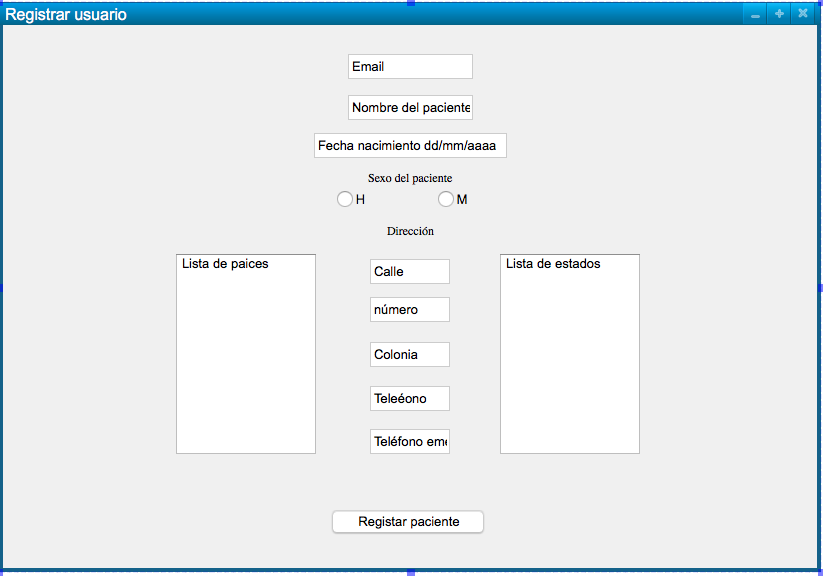
\includegraphics[width=0.8\textwidth]{images/UIRegPaciente}
        \caption{UIRegPaciente Pantalla registrar paciente}
    \end{figure}


\subsubsection{Entradas}
\begin{itemize}
\item Email del paciente: cadena de texto compuesta de 4 partes:  
            \begin{itemize}
                \item cadena de texto.
                \item carácter ‘@’
                \item cadena que identifica al servidor que brinda el servicio de correo electrónico
                \item carácter ‘.’ y dominio
            \end{itemize}
            \item Nombre completo del paciente:  3 cadenas de caracteres (Nombre(s), apellido paterno, apellido materno).
            \item Fecha de nacimiento del paciente: Fecha DD/MM/AAAA
            \item Sexo del paciente: 1 carácter . ‘H’ para hombre, ‘M’ para mujer.
            \item Dirección
            \begin{itemize}
                \item Calle: Cádena de caracteres.
                \item Número: Cádena de caracteres.
                \item Colonia: Cádena de caracteres.
                \item Estado: Cádena de caracteres.
                \item País : Cádena de caracteres.
                \item Teléfono particular: Cádena de 8 a 10 caracteres.
                \item Teléfono de emergencia: Cádena de 8 a 10 caracteres.
            \end{itemize}    
            \item Contraseña:  Cadena de longitud mínima de 8 caracteres

\end{itemize}

\subsubsection{Comandos}
\begin{itemize}
    \item \IUbutton{Registrar paciente}:  Verifica que los datos sean correctos. Si la verificación es correcta muestra \IUref{UI2}{Home}.  
\end{itemize}

\subsubsection{Mensajes}
    \begin{Citemize}
        \item {\bf MSG3a} “Datos incorrectos”.
        \item {\bf MSG3b} “Correo electrónico ya existente en la base de datos”.
    \end{Citemize}




\subsection{UI10ConsultExp Consultar expediente}

\subsubsection{Objetivo}
    Realizar la visualizacíón del expediente médifo del paciente. 

\subsubsection{Diseño}
   Esta pantalla aparece cuando el paciente da click en ``Mi expediente'' o el médico durante una consulta da click 
   en el nombre del paciente 

\begin{figure}[htbp!]
        \centering
            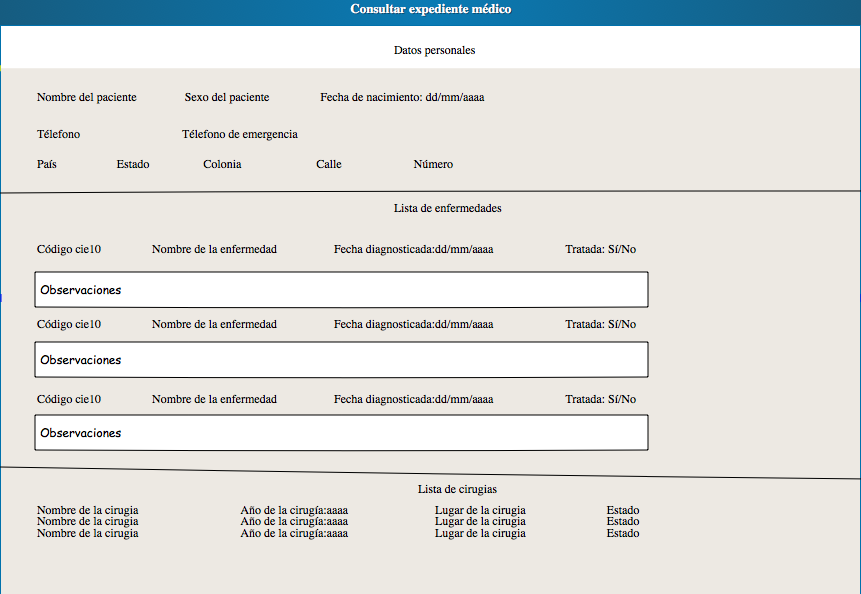
\includegraphics[width=0.8\textwidth]{images/UIEXP1}
            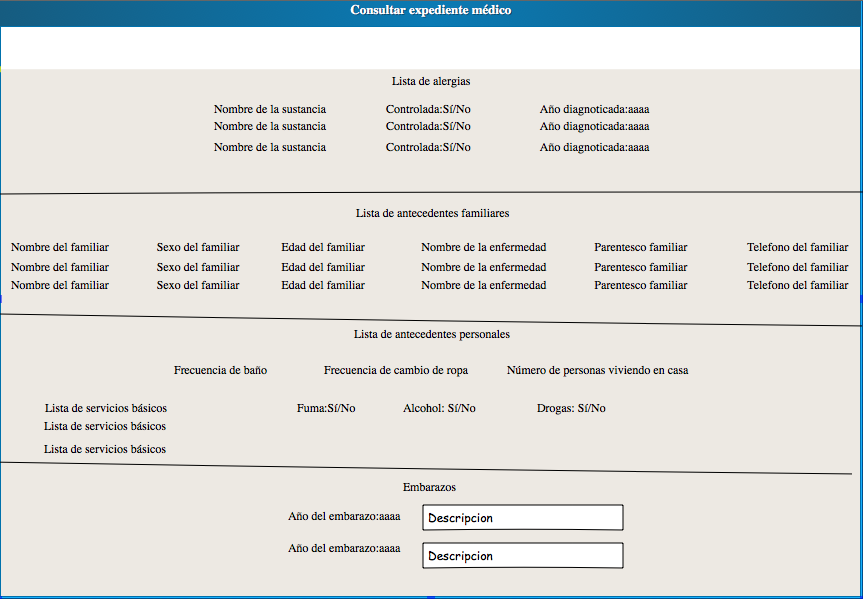
\includegraphics[width=0.8\textwidth]{images/UIEXP2}
            
    \end{figure}
\begin{figure}[htbp!]
        \centering
        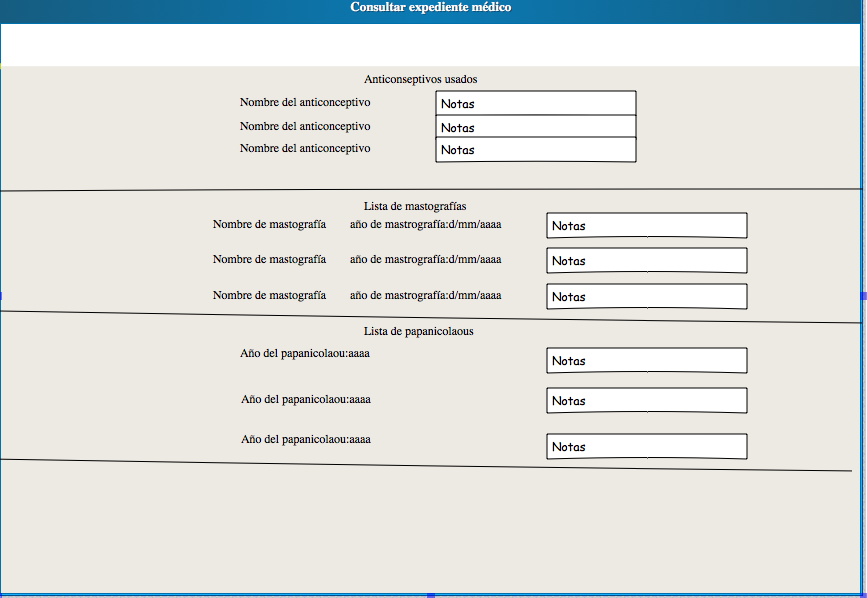
\includegraphics[width=0.8\textwidth]{images/UIEXP3}
            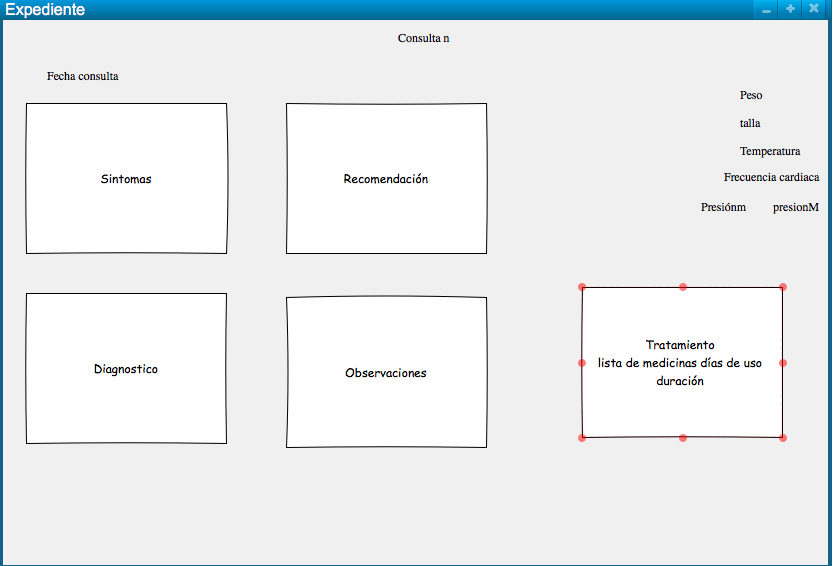
\includegraphics[width=0.8\textwidth]{images/UIEXP4}
        \caption{UIConsultExp Consultar expediente}
\end{figure}
\newpage
\subsubsection{Entradas}
\begin{itemize}
\item Ninguna
\end{itemize}

\subsubsection{Comandos}
\begin{itemize}
\item Ninguno
\end{itemize}

\subsubsection{Mensajes}
    \begin{Citemize}
        \item {\bf MSG3a} ``El paciente no cuenta con expediente médico''.
    \end{Citemize}


\subsection{UI7ConsultarVentasDiarias Consultar ventas diarias}
\subsubsection{Objetivo}
Poder tener un registro visual de las ventas que se han hecho en el día actual.
\subsubsection{Diseño}
   Esta pantalla aparece cuando el gerente da click en ``Consultar ventas diarias'' 


\begin{figure}[htbp!]
        \centering
            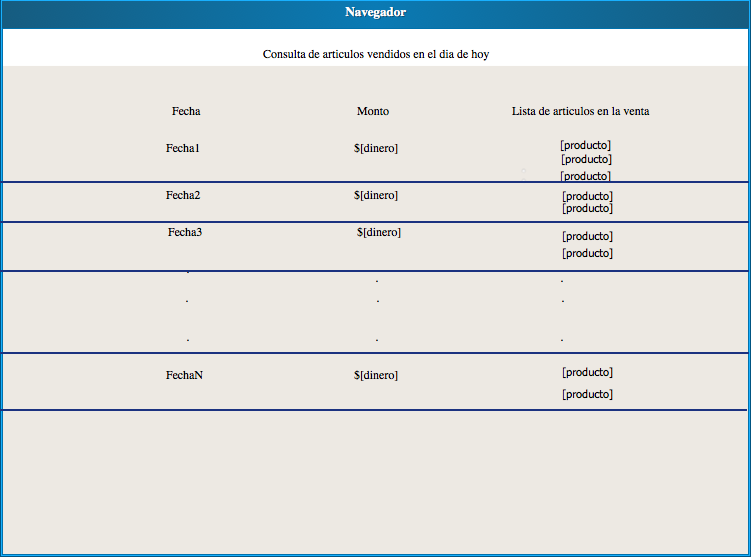
\includegraphics[width=0.8\textwidth]{images/consultaVentasDia}
            
            
    \end{figure}
    

\subsection{UI7ConsultarVentasMensuales Consultar ventas mensuales}
\subsubsection{Objetivo}
Poder tener un registro visual de las ventas que se han hecho en el mes actual.
\subsubsection{Diseño}
   Esta pantalla aparece cuando el gerente da click en ``Consultar ventas mensuales'' 


\begin{figure}[htbp!]
        \centering
            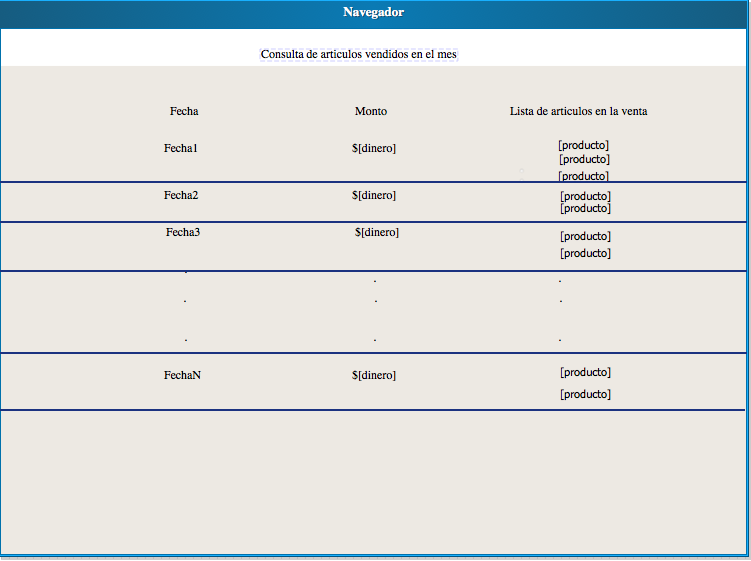
\includegraphics[width=0.8\textwidth]{images/consultaVentasMes}
            
            
    \end{figure}
    

\subsection{UI6ConsultarConsultasDiarias Consultar número de consultas diarias}
\subsubsection{Objetivo}
Poder tener un registro visual del número de consultas que ha dado el médico el día de hoy.
\subsubsection{Diseño}
   Esta pantalla aparece cuando el gerente da click en ``Consultar actividad diaria'' 


\begin{figure}[htbp!]
        \centering
            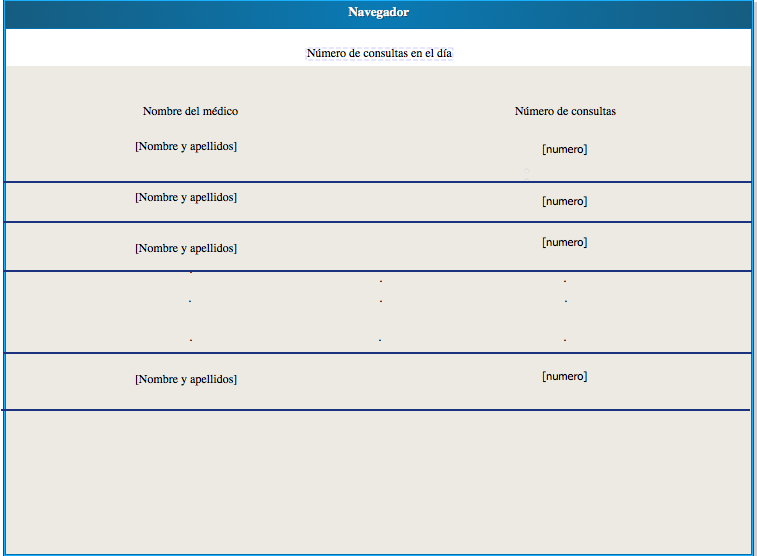
\includegraphics[width=0.8\textwidth]{images/consultaCitasDia}
            
            
    \end{figure}
 
 
 \subsection{UI6ConsultarConsultasMensuales Consultar número de consultas mensuales}
\subsubsection{Objetivo}
Poder tener un registro visual del número de consultas que ha dado el médico en el mes actual.
\subsubsection{Diseño}
   Esta pantalla aparece cuando el gerente da click en ``Consultar actividad mensual'' 


\begin{figure}[htbp!]
        \centering
            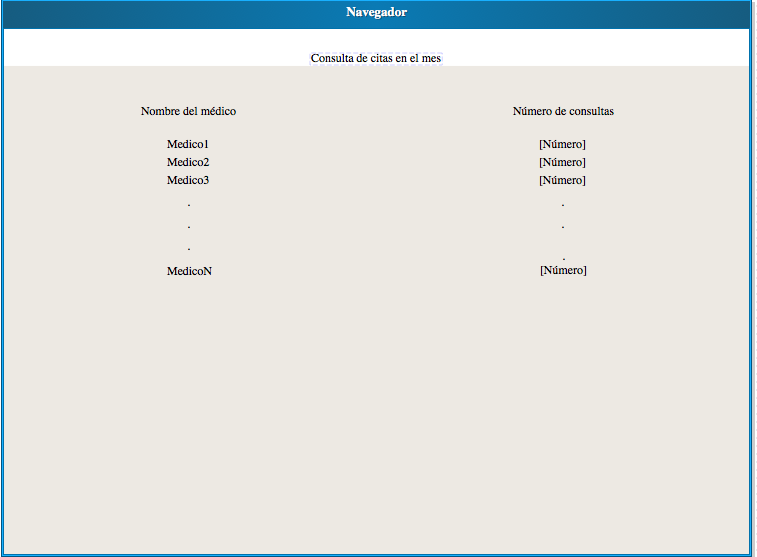
\includegraphics[width=0.8\textwidth]{images/consultaCitasMes}
            
            
    \end{figure}



Status API Training Shop Blog About
© 2016 GitHub, Inc. Terms Privacy Security Contact Help
